\chapter{Desarrollo de Colivi}
\label{chap:desarrollo_colivi}

A lo largo de este capítulo se presentará todo el proceso de desarrollo de ingeniería seguido desde la concepción de la idea inicial hasta la materialización completa de la plataforma, abordando tanto la arquitectura del servidor como la interfaz de usuario en sus vertientes web y adaptada a dispositivos móviles. El contenido comenzará con los aspectos preliminares de identidad corporativa, que abarcan el proceso de selección del nombre y el diseño del logotipo oficial. A continuación, se detallará el desarrollo del núcleo de servicios (\emph{backend}), el modelo de persistencia y seguridad, para posteriormente profundizar en la construcción del cliente web reactivo y su diseño adaptable.

\section{Identidad del proyecto: naming y diseño del logotipo}
\label{sec:identidad_proyecto}

Antes de iniciar la fase de codificación, resultó fundamental dotar al proyecto de una identidad verbal y visual coherente que sintetizara la propuesta de valor del sistema. La plataforma no debía percibirse como un mero portal transaccional de clasificados inmobiliarios, sino como un ecosistema integral pensado para facilitar la experiencia completa de habitar un piso compartido.

Inicialmente se exploraron diversas propuestas de denominación centradas de forma exclusiva en la búsqueda de alojamiento estudiantil (nombres provisionales como \emph{UniRooms}, \emph{FlatStudent} o \emph{PisoShare}). Sin embargo, estas alternativas se descartaron con rapidez por resultar excesivamente asépticas, impersonales y reduccionistas: omitían por completo el núcleo diferencial del software, que radica en la convivencia comunitaria cotidiana, el reparto equitativo de tareas y la gestión transparente de gastos entre compañeros.

Con el objetivo de reflejar adecuadamente la filosofía del \emph{co-living} universitario, se abordó un proceso de búsqueda que fusionara dos conceptos angulares:
\begin{itemize}
    \item El prefijo \textbf{``Co''}, derivado directo de \emph{co-living}, \emph{comunidad} y \emph{convivencia cooperativa}.
    \item La raíz verbal y fonética \textbf{``livi''}, procedente del término inglés \emph{living} (vivir, habitar, vida compartida).
\end{itemize}

De esta simbiosis léxica surgió la denominación definitiva: \textbf{Colivi}. Se trata de un nombre breve, eufónico y memorable, dotado de un carácter contemporáneo que comunica de inmediato la misión del proyecto: ``convivir y vivir juntos de forma sencilla y transparente''.

A partir de esta identidad verbal se concibió el diseño del logotipo corporativo, alineado con las especificaciones del sistema de diseño descritas en el capítulo anterior. Se persiguió una composición sobria y reconocible que integrara un isotipo geométrico representativo y el logotipo tipográfico. El isotipo estiliza la silueta protectora de un tejado y los pilares del hogar, entrelazando elementos que simbolizan la convergencia armónica de distintos miembros bajo un mismo espacio residencial. 

En cuanto a la armonía cromática, se aplicó rigurosamente la paleta maestra: el tono terracota cálido (\#C85A32) como color primario de marca —que transmite calidez de hogar, energía y hospitalidad— combinado con el azul marino profundo (\#0F172A) para la marca tipográfica, proyectando solidez estructural y rigor técnico.

El resultado final de esta identidad visual se exhibe a continuación en la figura \ref{fig:logo_colivi}.

\begin{figure}[H]
    \centering
    
\includegraphics[width=0.45\textwidth]{DesarrolloDeColivi/img/logo_colivi.png}
    \caption{Logotipo corporativo e imagotipo oficial de Colivi.}
    \label{fig:logo_colivi}
\end{figure}



\section{Desarrollo de la aplicación web y arquitectura de servicios}
\label{sec:desarrollo_web_servicios}

A lo largo de este capítulo se presentará todo el proceso de desarrollo seguido desde la concepción de la idea inicial hasta la finalización de ambas versiones de la aplicación: web y móvil. El contenido comenzará con aspectos preliminares como la elección del nombre y el diseño del logo. A continuación, se abordará en detalle el desarrollo de la versión web y, posteriormente, el de la versión móvil.

En esta sección del capítulo se describe el proceso de desarrollo de la versión web de **Colivi**. El proyecto se estructuró en dos capas principales: un frontend implementado con **Vite** y **React 19** (TypeScript), y un backend construido con **Spring Boot 3**, **Java 21** y **PostgreSQL 16**. La arquitectura adoptó el patrón de servicios desacoplados, separando claramente la lógica de negocio del acceso a datos y la presentación.

El desarrollo incluye la configuración del servidor local, la inserción de los datos iniciales, y la implementación de todas las vistas requeridas: inicio de sesión, registro, dashboard, perfil de usuario, explorador cartográfico de alojamientos, publicación de anuncios, gestión de gastos, cuadrante de tareas y asistencia mediante IA. Cada módulo se detalla en los sub‑apartados siguientes, organizados como archivos LaTeX independientes para cumplir con los principios SOLID.

\begin{figure}[H]
    \centering
    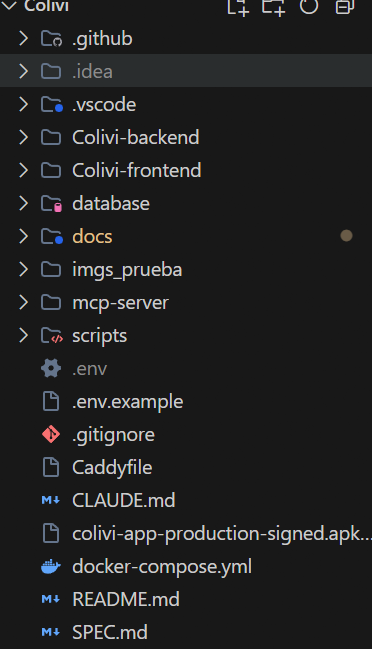
\includegraphics[width=0.92\textwidth]{DesarrolloDeColivi/img/estructura_proyecto.png}
    \caption{Estructura general del repositorio y partición modular del proyecto Colivi.}
    \label{fig:estructura_proyecto}
\end{figure}

\subsection{Creación del servidor local}
\label{subsec:creacion_servidor_local}

Para la creación del servidor local, lo primero que se tuvo que hacer fue crear una base de datos siguiendo el diagrama expuesto previamente en la sección 3.4. Una vez que la base de datos estuvo operativa en MySQL Workbench, se pudo comenzar con el desarrollo de las herramientas necesarias para garantizar su correcto funcionamiento dentro del proyecto.

El primer paso para conectar la base de datos al proyecto desarrollado en React fue la creación de los archivos de configuración. Entre ellos se encuentra el archivo .env, que contiene todas las variables necesarias para establecer la conexión con la estructura definida en MySQL Workbench, y el archivo db.js, encargado de realizar dicha conexión. Posteriormente, se creó el archivo server.js, que tiene la función de levantar el servidor local y definir las rutas necesarias.

Para llevar a cabo esta configuración fue necesario instalar una serie de dependencias fundamentales. En primer lugar, se utilizó la dependencia mysql2, que actúa como cliente de node.js para establecer la conexión con MySQL Workbench. También se empleó dotenv, una herramienta que permite cargar las variables definidas en el archivo .env. Otra dependencia esencial fue express, un framework de node.js que facilita la creación del servidor, la definición de rutas y la gestión de las peticiones HTTP. Finalmente, se incorporó cors, una utilidad que permite habilitar la comunicación entre el servidor backend y el frontend incluso cuando se ejecutan en puertos distintos.

Una vez completada esta configuración inicial, se procedió a la creación de los controladores (controllers), los modelos (models) y las rutas (routes) correspondientes para poder realizar las distintas consultas a la base de datos. Los modelos (models) se encargan de realizar las consultas en MySQL utilizando el lenguaje propio. Por su parte, los controladores (controllers) contienen la lógica de negocio que conecta las peticiones realizadas desde los endpoints definidos en las rutas con las consultas ejecutadas por los modelos. Finalmente, las rutas (routes) se encargan de definir los distintos endpoints para acceder a las funcionalidades del sistema desde el frontend.

Además, fue necesario conectar cada archivo de rutas correspondiente con el archivo server.js. Esto permite integrar todos los componentes del backend y garantizar que las peticiones que se realicen desde el frontend puedan ser gestionadas y procesadas correctamente.

\subsection{Patrones de diseño utilizados}
\label{subsec:patrones_diseno}

Además de la separación entre controladores, servicios y repositorios, la implementación de Colivi utiliza varios patrones de diseño clásicos. Su elección no responde únicamente a una clasificación teórica: cada patrón resuelve un problema concreto de variabilidad, coordinación o control del ciclo de vida del sistema.

\subsubsection{Patrón Strategy}

El patrón \emph{Strategy} permite seleccionar un algoritmo en tiempo de ejecución sin modificar el componente que solicita su ejecución. En Colivi se utiliza para asignar responsables a las tareas periódicas del hogar mediante dos modos de funcionamiento: asignación fija y rotación entre miembros.

La modalidad seleccionada determina qué miembro recibe cada tarea, pero el proceso general de creación y planificación permanece independiente del algoritmo concreto. De este modo, el sistema puede incorporar nuevas formas de asignación sin alterar los procesos principales.

El mismo criterio se aplica al almacenamiento de imágenes. La aplicación se apoya en una interfaz independiente del proveedor concreto, de manera que puede sustituirse Cloudinary u otro servicio externo sin modificar la gestión funcional de los alojamientos.

\subsubsection{Patrón Observer mediante eventos de Spring}

El patrón \emph{Observer} se utiliza para desacoplar las operaciones de negocio de las acciones posteriores que deben ejecutarse como consecuencia de dichas operaciones. Cuando una reserva, un gasto, una tarea o una denuncia cambia de estado, el componente productor comunica el acontecimiento al resto del sistema.

Los observadores reciben los cambios y ejecutan acciones secundarias independientes, como generar un registro en el muro de actividad o enviar una notificación. Estas acciones se procesan después de confirmar correctamente la operación principal, de forma que no se registre actividad de una modificación que haya sido revertida por un error.

Las áreas de reservas, mensajería y miembros del hogar siguen este modelo: convierten un cambio publicado por el dominio en una notificación o en una actualización secundaria. Los observadores pueden ampliarse con tareas independientes sin obligar al proceso principal a conocer los canales de salida concretos.

\subsubsection{Máquina de estados}

Las reservas y sus reglas de transición constituyen una máquina de estados explícita. Una solicitud comienza en estado pendiente y puede pasar, según su situación y quien realice la acción, a aceptada, confirmada, rechazada, cancelada o caducada.

Cada operación verifica el estado actual antes de cambiarlo. Por ejemplo, una solicitud solo puede confirmarse después de haber sido aceptada. Cancelar una solicitud rechazada o confirmar una solicitud todavía pendiente produce una excepción controlada. La máquina de estados incorpora también permisos por rol y validaciones transversales, como la prevención de solapamientos o la caducidad de reservas.

Una parte de esta responsabilidad se trata como un patrón \emph{State} de dominio en sentido estricto, mientras que el conjunto completo constituye una máquina de estados finitos. El estado no se representa mediante variables booleanas independientes, sino mediante un único estado con transiciones validadas dentro de la entidad y del servicio.

\subsubsection{Patrón Chain of Responsibility}

El acceso protegido al backend se implementa mediante una cadena de filtros de seguridad. El sistema establece primero las rutas públicas y las rutas que requieren autenticación, y después aplica sucesivamente las comprobaciones necesarias.

El primer filtro valida la identidad y construye el contexto de autenticación. Si la petición continúa, el siguiente filtro verifica que el usuario no esté baneado, eliminado o desactivado. Las peticiones rechazadas finalizan el procesamiento y las válidas pasan a la siguiente comprobación y, finalmente, al controlador solicitado.

Este patrón separa las responsabilidades criptográfica y de estado operativo. Añadir una política de seguridad nueva supone incorporar un filtro sin modificar los controladores ni las reglas existentes.

\subsubsection{Patrón Adapter y Proxy en el servidor MCP}

El servidor MCP actúa como adaptador entre dos protocolos. Una petición del protocolo MCP se traduce en la invocación de una herramienta, y cada herramienta delega en el servicio REST adecuado del backend.

El adaptador encapsula las llamadas HTTP y transforma respuestas y errores a operaciones coherentes con el protocolo MCP. Por tanto, las herramientas no necesitan conocer la implementación concreta del transporte HTTP.

El servidor también implementa una relación de tipo \emph{Proxy} o intermediario seguro: no almacena credenciales ni accede directamente a la base de datos. Reenvía la identidad del usuario en cada llamada y devuelve al protocolo MCP los errores de autenticación o autorización recibidos del backend. El control de pertenencia al hogar y de permisos continúa ejecutándose en la aplicación principal.

\subsubsection{Patrón Factory}

La construcción del servidor MCP encapsula la creación de sus componentes, el registro de herramientas y la selección del tratamiento de errores.

Esta aplicación del patrón \emph{Factory} evita que la capa de transporte o el enrutador HTTP construyan manualmente el servidor MCP en varios lugares. La fábrica permite además crear instancias con distintos catálogos de herramientas según el rol del usuario.

\subsubsection{Evaluación global de los patrones}

Estos patrones contribuyen a reducir el acoplamiento entre módulos y a mantener centralizadas las reglas susceptibles de cambiar. En particular, Strategy separa los algoritmos de asignación y almacenamiento, Observer desacopla las consecuencias secundarias del dominio, State limita las transiciones permitidas y Chain of Responsibility divide la autenticación y la autorización.

No todos los mecanismos del proyecto deben interpretarse como patrones adicionales. El uso de marcos de persistencia, la inyección por contenedor o el bloqueo optimista son implementaciones y mecanismos técnicos; no constituyen por sí solos nuevos patrones de diseño. Esta precisión evita atribuir al proyecto patrones que no aportan una decisión estructural diferenciada.

\subsection{Integración y consumo de APIs: arquitectura REST y servicios externos}
\label{subsec:integracion_apis}

En este apartado se detalla el flujo de comunicación y consumo de interfaces de programación de aplicaciones (APIs) implementado en Colivi, abarcando tanto la interacción entre el cliente web y el backend propio mediante arquitectura REST, como la integración con servicios públicos externos de geolocalización. El diseño persigue dos metas esenciales de ingeniería: garantizar contratos de datos estrictamente tipados y desacoplados, y optimizar el rendimiento minimizando las llamadas a servicios externos sujetos a restricciones de cuota.

\subsubsection{Consumo e integración de la API REST interna (Frontend -- Backend)}

La comunicación entre el cliente desarrollado en React y los microservicios transaccionales de Spring Boot se estructura sobre un protocolo RESTful sin estado (\emph{stateless}). Para evitar discrepancias de datos y fallos en tiempo de ejecución, se aplicó un principio de modelado simétrico entre los \emph{Data Transfer Objects} (DTOs) de Java y las interfaces tipadas de TypeScript en el cliente:

\begin{itemize}
    \item \textbf{Gestión de peticiones y mutaciones reactivas}: Las consultas de lectura (\texttt{GET}) y las operaciones de mutación (\texttt{POST}, \texttt{PUT}, \texttt{DELETE}) se gestionan a través de ganchos personalizados (\emph{custom hooks}) que encapsulan las funciones de \textbf{TanStack Query} (\texttt{useQuery} y \texttt{useMutation}). Esta capa intermedia proporciona un manejo automático de los estados del ciclo de vida asíncrono (\texttt{isLoading}, \texttt{isError}, \texttt{data}), evitando la duplicación de código en los componentes visuales.
    \item \textbf{Propagación de credenciales y autorización}: Mediante el interceptor de Axios, cada solicitud hacia rutas protegidas viaja acompañada de la cabecera estándar \texttt{Authorization: Bearer <JWT>}. El backend valida la firma criptográfica en el filtro de seguridad antes de despachar la petición al controlador de dominio pertinente.
    \item \textbf{Políticas de invalidación y actualización optimista}: Para garantizar una experiencia fluida al usuario, las mutaciones desencadenan la invalidación reactiva de claves de consulta específicas (\texttt{queryClient.invalidateQueries}). Por ejemplo, al registrar la liquidación de una deuda compartida en el hogar, el libro mayor contable y los saldos cruzados de todos los compañeros se sincronizan automáticamente en el cliente sin requerir una recarga completa de la página.
\end{itemize}

\subsubsection{Consumo de APIs externas y geocodificación (OpenStreetMap / Nominatim)}

Una de las funcionalidades nucleares de Colivi radica en la exploración de inmuebles sobre un mapa cartográfico en tiempo real. No obstante, los anfitriones y propietarios introducen la ubicación de sus viviendas mediante direcciones postales en lenguaje natural (calle, número, código postal y ciudad), las cuales no pueden ser interpretadas directamente por el motor cartográfico de Leaflet sin antes convertirse en coordenadas espaciales $(\text{latitud}, \text{longitud})$.

Para resolver esta necesidad se integró la API pública de geocodificación \textbf{Nominatim}, provista por la fundación \textbf{OpenStreetMap}. Sin embargo, este servicio externo impone una estricta Política de Uso Aceptable (\emph{Acceptable Use Policy}):
\begin{itemize}
    \item Un límite de tasa estricto (*Rate Limiting*) de \textbf{máximo 1 petición por segundo}.
    \item Prohibición expresa de ejecutar consultas masivas o búsquedas repetitivas para una misma dirección.
    \item Requerimiento obligatorio de cabecera \texttt{User-Agent} identificativa para monitorizar el consumo del servicio.
\end{itemize}

Si la aplicación web consultara la API externa de Nominatim cada vez que un usuario explora el mapa o desplaza el zoom, el sistema colapsaría de inmediato al superar los límites de tasa, acarreando el bloqueo de la dirección IP del servidor y generando una latencia inasumible en la interfaz.

Para sortear esta limitación y garantizar la máxima eficiencia, se implementó una estrategia de \textbf{geocodificación asíncrona con persistencia local}:

\begin{enumerate}
    \item \textbf{Resolución única durante el alta del inmueble}: Cuando el anfitrión publica o actualiza un alojamiento, el backend captura la dirección estructurada y ejecuta una única llamada controlada al servicio de Nominatim.
    \item \textbf{Persistencia de coordenadas en base de datos}: La respuesta JSON de la API externa es procesada y las coordenadas resultantes se almacenan permanentemente en las columnas \texttt{latitude} y \texttt{longitude} de la tabla relacional \texttt{accommodations} de PostgreSQL.
    \item \textbf{Consultas locales indexadas}: En las búsquedas habituales del cliente web, la plataforma no realiza ninguna llamada a Nominatim; las viviendas se consultan directamente desde la base de datos local mediante índices numéricos sobre las coordenadas geográficas, sirviendo los datos con tiempos de respuesta inferiores a 20~ms y respetando rigurosamente los términos de uso del proveedor libre.
\end{enumerate}

\subsubsection{Verificación inicial de contratos y datos de prueba}

Con el fin de verificar la robustez de los contratos de la API REST y certificar visualmente la renderización de las coordenadas en el mapa cartográfico sin depender de inserciones manuales tediosas durante el desarrollo, se diseñó una inicialización automatizada de datos de prueba (\emph{seed data}). Esta se articula mediante una migración determinista en Flyway (\texttt{V999\_\_insert\_dev\_seed\_data.sql}) que preconfigura usuarios maestros y hogares de convivencia con cláusula \texttt{ON CONFLICT DO NOTHING}, complementada por un script en Python (\texttt{seed\_db.py}) que simula la interacción de anfitriones publicando inmuebles geolocalizados en los distritos universitarios más representativos de España (Madrid, Barcelona, Granada, Salamanca, Sevilla y Valencia).


\subsection{Inicio de sesión, registro y autenticación}
\label{subsec:autenticacion_registro}

En esta primera fase del desarrollo web se implementaron los flujos de **login** y **registro** siguiendo los lineamientos de seguridad y usabilidad descritos por el equipo. El frontend, construido con **React 19** y **TypeScript**, dispone de las vistas `LoginPage.tsx`, `RegisterPage.tsx` y `ResetPasswordPage.tsx`. Cada formulario está gestionado mediante **React Hook Form** y validado con **Zod**, garantizando requisitos de contraseñas (mínimo 8 caracteres, mayúsculas, dígitos y símbolos) y formatos de correo electrónico.

El backend, basado en **Spring Boot 3**, expone los endpoints `/api/v1/auth/login` y `/api/v1/auth/register`. La autenticación es **stateless**, utilizando **JWT** firmado con HMAC‑SHA256. Los tokens se envían al cliente y se almacenan en `localStorage`, siendo añadidos automáticamente a todas las peticiones subsecuentes mediante un interceptor de **Axios**.

Para la recuperación de credenciales se implementó el flujo de *reset password*: el usuario solicita un enlace temporal que contiene un token de un solo uso, el cual permite establecer una nueva contraseña sin revelar la anterior.

En el nivel de seguridad del backend, **Spring Security 6** administra un filtro `JwtAuthenticationFilter` que valida cada petición bajo `/api/v1/**`, rechaza cuentas suspendidas y gestiona la autorización basada en roles (`ADMIN`, `MEMBER`).

\subsection{Panel de control (Dashboard) y gestión de la convivencia}
\label{subsec:dashboard_convivencia}

El panel de control principal representa el centro neurálgico de la experiencia diaria del estudiante o inquilino en Colivi. Tras autenticarse, la plataforma presenta una vista consolidada que centraliza el estado actual de la convivencia residencial, los compromisos económicos compartidos y la distribución de responsabilidades domésticas.

\subsubsection{Estructura de la interfaz y composición de widgets}

En el frontend, el panel de control se implementa a través del componente de página principal (\texttt{HomePage.tsx}) y componentes de agregación modular en \texttt{components/layout/}:

\begin{itemize}
    \item \textbf{Encabezado de comunidad y membresía activa}: Muestra el nombre del hogar actual (por ejemplo, \emph{«Piso Estudiantes Centro»}), la insignia identificativa de rol del usuario (\texttt{ADMIN} o \texttt{MEMBER}) y la lista interactiva de compañeros de piso con sus respectivos avatares y códigos de color personalizados, facilitando la distinción visual instantánea.
    \item \textbf{Widget de balance financiero rápido}: Sintetiza el saldo neto del usuario en el piso. Si el balance es positivo, indica el importe total que sus compañeros le adeudan; si es negativo, alerta en tono de énfasis sobre los pagos pendientes, ofreciendo un botón de acceso directo a la liquidación.
    \item \textbf{Widget de tareas domésticas inminentes}: Expone las labores asignadas al usuario para la semana en curso (como la limpieza de zonas comunes o retirada de residuos), permitiendo marcar tareas como finalizadas con un solo clic o solicitar un «rescate» gamificado a la comunidad.
    \item \textbf{Gestión de invitaciones del hogar}: Para los administradores de la vivienda, el panel proporciona un botón para copiar al portapapeles o regenerar el código de invitación alfanumérico (ejemplo: \texttt{PISO-CENTRO-2024}), permitiendo la adhesión inmediata de nuevos inquilinos sin requerir trámites administrativos complejos.
\end{itemize}

\subsubsection{Agregación de datos y optimización de consultas en backend}

Para evitar el problema clásico de sobrecarga por múltiples peticiones HTTP en cascada (*Waterfall Requests*), el backend expone un endpoint consolidado en \texttt{HomeController} (\texttt{GET /api/v1/homes/{homeId}/summary}):

\begin{enumerate}
    \item \textbf{Consolidación en un único DTO (\texttt{HomeSummaryDTO})}: El servicio \texttt{HomeService} orquesta en una única transacción de sólo lectura la recopilación de los miembros activos del hogar, los últimos tres gastos registrados, el balance contable individual del solicitante y el cuadrante de tareas activas.
    \item \textbf{Prevención de consultas N+1 en Hibernate}: Se diseñaron consultas especializadas en \texttt{HomeRepository} empleando cláusulas \texttt{LEFT JOIN FETCH} sobre las entidades relacionadas (\texttt{members}, \texttt{expenses}, \texttt{chores}), asegurando que la base de datos PostgreSQL resuelva toda la información en un número acotado de consultas SQL altamente optimizadas.
    \item \textbf{Sincronización reactiva con TanStack Query}: En el cliente, la consulta del panel se suscribe a una clave de caché unificada (\texttt{['home', homeId, 'summary']}). Cuando cualquier miembro del piso añade un gasto o completa una tarea, las mutaciones invalidan selectivamente esta clave, provocando un refresco en segundo plano que mantiene la interfaz siempre actualizada sin saltos visuales ni parpadeos.
\end{enumerate}


\subsection{Perfil de usuario y gobernanza de cuenta}
\label{subsec:perfil_usuario}

El perfil de usuario constituye la carta de presentación de inquilinos y propietarios dentro del ecosistema Colivi. Permite gestionar la identidad digital del estudiante, sus preferencias de convivencia, su historial de reservas y el ciclo de vida de su cuenta.

\subsubsection{Diseño de la vista y componentes de configuración}

En el cliente web, la funcionalidad se distribuye entre la vista de perfil privado (\texttt{ProfilePage.tsx}) y la ficha pública de presentación (\texttt{PublicProfilePage.tsx}):

\begin{itemize}
    \item \textbf{Gestión de información personal y de contacto}: El usuario puede modificar su nombre, apellidos, biografía descriptiva y teléfono móvil. La entrada de datos está blindada mediante esquemas de validación que aseguran que los números sigan el estándar internacional E.164.
    \item \textbf{Generación de avatares e identidad visual}: Para usuarios que no suben una fotografía propia, se integra un generador determinista de avatares vectoriales basado en las iniciales y el alias del usuario, utilizando la paleta cromática corporativa para mantener una estética armónica en toda la plataforma.
    \item \textbf{Ficha de reputación y perfil público}: Al evaluar solicitudes de reserva o buscar nuevos compañeros de piso, los usuarios pueden consultar el perfil público de otros miembros. Dicha vista expone las valoraciones medias recibidas en estancias previas, las insignias de verificación (correo confirmado, teléfono verificado) y los intereses de convivencia (hábitos de estudio, compatibilidad con mascotas, horarios de descanso).
    \item \textbf{Desactivación voluntaria y derecho al olvido}: Siguiendo los principios de privacidad y cumplimiento del RGPD, el usuario puede desactivar temporalmente su perfil o solicitar el borrado de sus datos personales. Al desactivar la cuenta, el sistema oculta sus publicaciones y cancela automáticamente sus solicitudes pendientes.
\end{itemize}

\subsubsection{Lógica de servicio y seguridad de perfiles en backend}

En el backend, el servicio \texttt{UserService} y el controlador \texttt{UserController} gestionan las transiciones de estado y la integridad de los datos:

\begin{enumerate}
    \item \textbf{Validación de unicidad y control de concurrencia}: La actualización del correo electrónico o del alias requiere comprobaciones de unicidad en base de datos. Para evitar colisiones en entornos concurrentes, las operaciones de actualización se ejecutan bajo transacciones atómicas con aislamiento de lectura comprometida.
    \item \textbf{Sanitización de contenidos}: Las biografías y campos de texto libre introducidos por el usuario se someten a un proceso de sanitización para neutralizar cualquier intento de inyección de código malicioso (\emph{Cross-Site Scripting}, XSS).
    \item \textbf{Ciclo de reactivación mediante token firmado}: Cuando un usuario inactivo intenta iniciar sesión, el sistema genera un token criptográfico de reactivación vinculado a la tabla \texttt{reactivation\_tokens} con un periodo de validez de 24 horas, despachando un correo transaccional automático para confirmar la reapertura de la cuenta.
\end{enumerate}


\subsection{Explorador cartográfico y catálogo de alojamientos}
\label{subsec:explorador_alojamientos}

El explorador cartográfico es la herramienta principal mediante la cual los estudiantes descubren y comparan opciones de alojamiento residencial. Diseñada bajo un patrón de panel dividido (*Split-Screen Layout*), la interfaz combina la potencia visual de un mapa interactivo con la riqueza descriptiva de un catálogo de tarjetas inmobiliarias.

\subsubsection{Construcción del visor interactivo en frontend}

En el cliente web, esta pantalla se articula en el componente MapSearchPage.tsx, apoyado en la suite geoespacial de \textbf{Leaflet}, \textbf{React-Leaflet} y \textbf{Supercluster}:

\begin{itemize}
    \item \textbf{Disposición dividida y desplazamiento independiente}: La pantalla se divide en dos columnas ergonómicas. En el lado izquierdo (o panel superior en dispositivos móviles), se presenta el mapa cartográfico interactivo que permanece anclado a la altura de la ventana; en el lado derecho, se despliega la rejilla con las tarjetas de los inmuebles disponibles, dotada de desplazamiento vertical aislado (overflow-y: auto). Al pasar el cursor sobre una tarjeta, el marcador correspondiente en el mapa se ilumina automáticamente mediante una transición visual.
    \item \textbf{Agrupación por conglomerados espaciales (\emph{Supercluster})}: Para garantizar un rendimiento óptimo de 60 cuadros por segundo al manipular el mapa, los puntos de alojamiento no se renderizan individualmente si su densidad es alta. La biblioteca Supercluster calcula en memoria los grupos de marcadores según el nivel de zoom actual y los límites geográficos visibles (*Bounding Box*), mostrando insignias numéricas que se disuelven dinámicamente al acercar el mapa.
    \item \textbf{Filtrado reactivo con retardo controlado (\emph{Debounce})}: La barra de herramientas permite filtrar viviendas por ciudad, rango de precios, tipo de alquiler (habitación privada o piso completo), número de baños y comodidades indispensables (\emph{amenities} como calefacción, ascensor, aire acondicionado o conexión a internet). Para evitar saturar el servidor con peticiones innecesarias mientras el usuario escribe en la barra de búsqueda o ajusta el control deslizante de precio, se aplica una técnica de retardo (*debounce*) de 300~ms mediante lodash.debounce.
\end{itemize}

\subsubsection{Motor de búsqueda geoespacial y paginación en backend}

En el backend, las peticiones de búsqueda convergen en el método search() de AccommodationController:

\begin{enumerate}
    \item \textbf{Filtrado dinámico con especificaciones JPA}: Se implementó un constructor de consultas basado en \textbf{Spring Data JPA Specifications} (JpaSpecificationExecutor). Este patrón compone dinámicamente predicados SQL en función de los parámetros recibidos en la consulta HTTP (city, minPrice, maxPrice, amenities), evitando la concatenación manual de cadenas y blindando el endpoint contra inyecciones SQL.
    \item \textbf{Filtrado por cuadrante geográfico}: Cuando el usuario navega o desplaza el mapa, el cliente envía las coordenadas de las esquinas del área visible (northEastLat, northEastLng, southWestLat, southWestLng). La consulta en base de datos aplica restricciones espaciales de acotamiento (BETWEEN), retornando únicamente las viviendas que se encuentran dentro del cuadrante proyectado.
    \item \textbf{Paginación y proyección optimizada}: Para minimizar el ancho de banda transferido, la respuesta no incluye la entidad completa con todas sus fotos y relaciones, sino un DTO ligero (ListingCardDTO) que contiene únicamente el título, precio mensual, coordenadas y la fotografía de portada principal.
\end{enumerate}


\subsection{Publicación de inmuebles y ciclo de reservas}
\label{subsec:publicacion_reservas}

El módulo inmobiliario y de contratación rige el ciclo de vida mediante el cual los propietarios publican sus anuncios y los estudiantes formalizan solicitudes de alquiler vinculadas a un depósito o fianza.

\subsubsection{Formulario multi-paso y gestión multimedia en frontend}

Para maximizar la tasa de finalización del alta de una vivienda, el cliente web estructura el proceso a través del componente AccommodationFormPage.tsx mediante un asistente por etapas (*Multi-Step Wizard*):

\begin{itemize}
    \item \textbf{Etapa 1 -- Localización y geocodificación}: El anfitrión introduce los datos postales de la vivienda. La interfaz valida la dirección en tiempo real y muestra una previsualización de confirmación sobre el mapa interactivo.
    \item \textbf{Etapa 2 -- Características físicas y comodidades}: Se registran la superficie en metros cuadrados, el número de dormitorios, baños disponibles y el equipamiento del piso mediante selectores accesibles (*tags* de selección múltiple).
    \item \textbf{Etapa 3 -- Galería fotográfica y selección de portada}: El usuario puede subir múltiples fotografías en alta definición. Mediante la tabla asociativa listing_image_selection, el sistema permite ordenar las imágenes mediante arrastrar y soltar (*drag and drop*) y elegir cuál actuará como imagen principal de portada para el catálogo público.
    \item \textbf{Etapa 4 -- Condiciones contractuales y fianza}: Se fija el precio mensual del alquiler y el importe obligatorio de la fianza legal en garantía de conservación de la vivienda.
\end{itemize}

\subsubsection{Máquina de estados de reserva y control de concurrencia en backend}

La interacción contractual entre inquilino y anfitrión está gobernada por una máquina de estados estricta implementada en BookingRequestService:

\begin{enumerate}
    \item \textbf{Transiciones de estado formales}: Una solicitud de reserva nace en estado PENDING al ser enviada por el estudiante. El propietario dispone de un plazo temporal acotado para tomar una decisión: si la acepta, transiciona a ACCEPTED; si la declina, pasa a REJECTED; y si expira el plazo máximo sin respuesta, un proceso programado la marca automáticamente como EXPIRED.
    \item \textbf{Prevención de sobre-reserva mediante bloqueo optimista (\emph{Optimistic Locking})}: Para evitar que dos estudiantes reserven simultáneamente la misma habitación disponible en un entorno concurrido, la entidad Accommodation incorpora un campo de versión anotado con @Version. Si dos transacciones intentan confirmar la reserva al mismo instante, Hibernate detecta la colisión de versiones arrojando una excepción de concurrencia optimista (OptimisticLockException), abortando la segunda operación de forma segura y protegiendo la integridad del inventario.
    \item \textbf{Bloqueo y custodia de fianza}: Cuando una solicitud es aceptada, el sistema genera el registro financiero de la fianza en la tabla booking_requests, asociando un identificador de transacción y asegurando que las partes cuenten con un respaldo económico antes de formalizar la entrega de llaves.
\end{enumerate}


\subsection{Gestión financiera y liquidación de gastos compartidos}
\label{subsec:gestion_gastos}

La gestión contable de gastos es uno de los principales focos de fricción en la convivencia entre estudiantes. Colivi resuelve esta problemática mediante un libro mayor digital transparente que registra las compras comunes y simplifica automáticamente los pagos entre compañeros de piso.

\subsubsection{Interfaz contable y desglose de cuotas en frontend}

En el cliente web, la funcionalidad se centraliza en el componente de página \texttt{ExpensesPage.tsx} y sus modales asociados:

\begin{itemize}
    \item \textbf{Formulario de registro de gasto compartido}: Permite ingresar la descripción del gasto (ejemplo: «Compra semanal Mercadona» o «Factura de suministro eléctrico»), el importe total pagado en euros y el selector del pagador. El usuario puede elegir entre dividir el coste equitativamente entre todos los miembros activos del hogar o seleccionar participantes individuales con importes asignados personalizados.
    \item \textbf{Panel visual de saldos cruzados y matriz de deudas}: La vista calcula en tiempo real el saldo neto de cada compañero respecto al resto de la comunidad. Los balances se representan con código de colores: verde para saldos acreedores (dinero a recibir) y rojo para saldos deudores (dinero a abonar).
    \item \textbf{Modal de liquidación y pago entre miembros}: Al hacer clic en «Saldar deuda», se abre un formulario de liquidación donde un miembro registra una transferencia hacia otro compañero. La interfaz valida que el importe abonado no exceda la deuda acumulada pendiente.
\end{itemize}

\subsubsection{Motor contable y consistencia transaccional en backend}

En el backend, el procesamiento financiero se aloja en \texttt{ExpenseService} y se ejecuta bajo estrictas garantías transaccionales:

\begin{enumerate}
    \item \textbf{Transaccionalidad ACID atómica (\texttt{@Transactional})}: El registro de un gasto implica insertar la cabecera en \texttt{home\_expenses} y simultáneamente las cuotas desglosadas en \texttt{home\_expense\_participants}. Si ocurre cualquier fallo o la suma de las partes no coincide con el importe global, la anotación \texttt{@Transactional} de Spring revierte automáticamente todos los cambios en PostgreSQL, impidiendo descuadres contables.
    \item \textbf{Algoritmo de simplificación de deudas}: El servicio implementa un algoritmo de compensación de saldos que reduce la complejidad de las transferencias. Si el inquilino $A$ debe $20$~€ a $B$, y $B$ debe $20$~€ a $C$, el sistema calcula que $A$ abone directamente los $20$~€ a $C$, eliminando transacciones redundantes entre los convivientes.
    \item \textbf{Registro histórico y trazabilidad de pagos}: Cada pago de liquidación se persiste en la tabla \texttt{home\_expense\_payments}, dejando constancia inmutable de la fecha, el emisor, el receptor y la cantidad transferida, lo que alimenta el muro de actividad del hogar para auditoría interna de los compañeros.
\end{enumerate}


\subsection{Cuadrante de tareas domésticas y asistente inteligente}
\label{subsec:tareas_asistente}

El último eslabón funcional de la plataforma aborda la organización del trabajo doméstico compartido y la integración de un asistente conversacional inteligente para dar soporte autónomo a la comunidad.

\subsubsection{Cuadrante rotativo de tareas y gamificación}

Para erradicar los desacuerdos derivados del reparto desigual de tareas de limpieza y mantenimiento, Colivi implementa en \texttt{ChoresPage.tsx} un planificador automatizado respaldado por un sistema de recompensas:

\begin{itemize}
    \item \textbf{Series recurrentes y rotación Round-Robin}: El administrador del hogar define las tareas periódicas (ejemplo: «Limpieza de cocina los domingos» o «Tirar la basura reciclable»). El motor del backend distribuye los turnos de forma secuencial y equitativa entre los miembros activos del piso mediante un algoritmo rotativo \emph{Round-Robin}, garantizando que la carga de trabajo se distribuya de manera perfectamente homogénea a lo largo del curso académico.
    \item \textbf{Mecánica gamificada de «Rescate de tareas»}: Durante periodos de alta exigencia académica (como épocas de exámenes finales), un estudiante puede encontrarse imposibilitado para ejecutar su turno asignado. En lugar de generar conflictos, el sistema permite activar un botón de «Solicitar rescate». Cualquier otro compañero de piso puede asumir la tarea voluntariamente a cambio de recibir puntos de karma de la comunidad, incentivando la cooperación solidaria.
    \item \textbf{Verificación y puntuación acumulativa}: Al completar una labor, el usuario la marca como realizada, actualizando su puntuación en la tabla clasificatoria del hogar y registrando la acción en el muro de trazabilidad común.
\end{itemize}

\subsubsection{Canal de mensajería contextual y copiloto inteligente con protocolo MCP}

La comunicación y el soporte se articulan en el frontend mediante la bandeja de mensajes (\texttt{MessagesPage.tsx}) y el widget del asistente inteligente:

\begin{enumerate}
    \item \textbf{Chat directo contextual}: Permite la conversación privada entre inquilinos y propietarios para pactar visitas, así como un canal grupal interno exclusivo para los miembros del hogar.
    \item \textbf{Asistente conversacional contextual}: Integrado en la interfaz mediante \textbf{Spring AI}, el usuario puede interactuar en lenguaje natural con un copiloto inteligente. Dicho asistente no se limita a responder preguntas estáticas, sino que está conectado a las herramientas del backend mediante el protocolo estándar \textbf{Model Context Protocol (MCP)} desarrollado en el directorio \texttt{mcp-server/}.
    \item \textbf{Orquestación segura de herramientas}: Cuando el usuario consulta al asistente cuestiones como «¿Cuánto dinero debo en el piso?» o «¿A quién le toca limpiar el baño esta semana?», el modelo de lenguaje selecciona e invoca dinámicamente las herramientas correspondientes (\texttt{getPendingDebts}, \texttt{getChoreSchedule}). Para preservar la privacidad entre hogares, la ejecución de cada herramienta exige un ticket de sesión temporal que acota estrictamente la consulta a los datos del piso al que pertenece el usuario.
\end{enumerate}



